%% LyX 2.3.1 created this file.  For more info, see http://www.lyx.org/.
%% Do not edit unless you really know what you are doing.
\documentclass[a4paper,english,doc]{apa6}
\usepackage[T1]{fontenc}
\usepackage[latin9]{inputenc}
\usepackage{color}
\usepackage{babel}
\usepackage{graphicx}
\usepackage[unicode=true,pdfusetitle,
 bookmarks=true,bookmarksnumbered=false,bookmarksopen=false,
 breaklinks=false,pdfborder={0 0 0},pdfborderstyle={},backref=false,colorlinks=true]
 {hyperref}

\makeatletter

%%%%%%%%%%%%%%%%%%%%%%%%%%%%%% LyX specific LaTeX commands.
\special{papersize=\the\paperwidth,\the\paperheight}

%% Because html converters don't know tabularnewline
\providecommand{\tabularnewline}{\\}

%%%%%%%%%%%%%%%%%%%%%%%%%%%%%% Textclass specific LaTeX commands.
\usepackage[natbibapa]{apacite}

%%%%%%%%%%%%%%%%%%%%%%%%%%%%%% User specified LaTeX commands.
\usepackage[table]{xcolor}

\makeatother

\begin{document}
\title{Predicting the urgency of urban issues}
\author{Christian Braz}
\leftheader{Author}
\affiliation{George Washington University\\
Department of Data Science}
\abstract{City maintenance is laborious and expensive. One of the main challenges
is to monitor unpredictable situations like potholes, grafiti, broken
footpaths, and so on. Once detected, government officials must be
able to allocate the resources timely and prioritizing the issues
most relevant for the citizens. The pervasive presence today of mobile
internet connection in urban centers has enabled modern ways of interaction
between the municipality and the population, resulting in the so-called
Government 2.0. One of such way is crowdsourcing platforms, such as
See-Click-Fix, FixMyStreet, CitySourced, OpenIDEO, and many others,
which allow and stimulate collaborative participation by reporting
urban issues. The importance of an issue can be endorsed via votes
in the platform, meaning that issues with more votes represent the
overall felling of the neighborhood that those should be solved first.
This, in turn, constitutes important information to help organizing
logistics, allocate resources, and fulfill citizens' well-being feeling.
The problem is that may take time until collecting enough votes to
be able to estimate the urgency of an issue. In this work we propose
to estimate the number of votes an issue will receive using machine
learning techniques. As the number of votes is a proxy to the urgency,
we hope to improve city maintenance by providing in advance sensitive
information. }
\keywords{crowdsourcing, government 2.0, web 2.0, machine learning }
\maketitle

\section{Introduction}

Since its rising in early 90s, the World Wide Web has been modifying
the way people interact. Its distributed infrastructure, built upon
Internet's top layers, made it pervasive and an ideal tool to enable
all kinds of communications services. On a business perspective, new
jargons were created trying to categorize such virtual interactions,
such as Business-to-Consumer, Business-to-Bussiness, and Customer-to-Customer
\citep{B2B}. Social networks are also an example of interaction.
Facebook, Twitter or Instagram are well known interactive platforms
which enable users express their opinions. Governments have also been
experimenting changes in the way the citizens interact with them and
Kanhere (2011) provides a comprehensive overview. The so-called Government
2.0 implies that information should flow not only from the government
to the citizens but also from citizens to the government and among
citizens. 

City maintenance is expensive, since it involves monitoring and fixing
a variety of complex issues related to public safety, environmental
problems, and quality of life. In particular, monitoring unpredictable
urban issues (e.g., potholes, damaged street signs, graffiti, street
light issues, damaged trees) usually requires a large number of employees
working on a permanent basis. However, these same urban centers are
full of people armed with their GPS enabled cell phones, and represent
an important asset to help fine-grained monitoring capabilities. Civic
engagement platforms, such as See-Click-Fix.com, allow citizens to
report urban issues by entering, for instance, GPS location and free
text describing the problem. Having this information, in turn, helps
municipalities to reduce costs and improve logistics by better allocating
resources.

Another important aspect in city maintenance, is how to rank the problems.
As the resources are limited, most of the time would not be possible
to fix all the open issues. Thus, it is necessary to have a way to
measure which ones are more important. In the same crowdsourcing platforms,
the importance of an issue can be endorsed via votes, meaning that
the number of votes can act as a proxy to the urgency of an issue.
Therefore, a rank of issues can be built based on those votes. While
the number of votes an issue receives ultimately reflects its urgency
to be solved, acquiring a significant number of votes may take several
days or weeks, leading to ineffectiveness and late responses. In order
to become more responsive and better meet the needs and concerns of
the citizens, government officials must be able to prioritize more
urgent issues as soon as possible. 

In this work, we evaluate machine learning techniques to predict the
number of votes an issue will receive. More specifically, we evaluate
Ridge Regression, Support Vector Machine (SVM), and Long Short Term
Memory (LSTM) algorithms. We hope to demonstrate the feasibility of
this approach, and help to contribute in modernizing an important
aspect of public administration. This wok is organized as follows:
next we expose more details about the problem and the data, then we
describe the experiment and show the results, and finally we address
our final considerations. 

\section{Problem statement and the data}

Our experiments use the {[}SeeClickFix{]} hackathon data, comprising
34 Mb of size and consisting of a total of 223,129 reported issues
from four cities: Oakland, Richmond, New Haven, and Chicago. SeeClickFix.com
is a crowdsourcing initiative that allows citizens to report issues
categorized in 311 different types. The main way to submit a request
is taking a picture and sending it via their mobile app. They claim
that the service manages the whole work-flow, linking the citizen
with the city hall. 

Table 1 shows a description of the data. There are eleven attributes,
being five of them (in bold) used as predictors, and \emph{num\_votes}
as the target variable. Notice the high rate of missing value for
\emph{tag\_type}. It will be used to produce a baseline model, but
not for predictions. Figure 1, 2, and 3 show the distribution of the
records among issue categories (only 24\% of the data). 

\begin{table}
\begin{centering}
\begin{tabular}{|c|c|c|c|}
\hline 
\textbf{Column} & \textbf{Description} & \textbf{Type} & \textbf{\% Missing Values}\tabularnewline
\hline 
\hline 
id & randomly assigned id & Numeric & 0\tabularnewline
\hline 
\textbf{latitude}  & latitude of the issue & Numeric & 0\tabularnewline
\hline 
\textbf{longitude} & longitude of the issue & Numeric & 0\tabularnewline
\hline 
\textbf{summary} & short text title & Text & 0\tabularnewline
\hline 
\textbf{description} & longer text explanation & Text & 52\tabularnewline
\hline 
\textbf{date} & yyyy-mm-dd HH:mm:ss  & Timestamp & 0\tabularnewline
\hline 
num\_comments  & number of user comments & Numeric & 0\tabularnewline
\hline 
num\_views & number of views & Numeric & 0\tabularnewline
\hline 
source & where the issue was created & Categorical & 13\tabularnewline
\hline 
tag\_type & type of issue & Categorical & 76\tabularnewline
\hline 
\textbf{num\_votes} & number of user votes & Numeric & 0\tabularnewline
\hline 
\end{tabular}
\par\end{centering}
\caption{Dataset summary}

\end{table}
In Figure 1 we can see that issues related to trash, trees and potholes
correspond to more than 50\% of all issues, whereas issues related
to lost and found items, or to public art, are rarely reported by
citizens. Issues reported more frequently have higher absolute number
of votes. But this absolute number is not very useful. Figure 2 gives
an insight about the urgency of an issue by computing the average
of votes by category. We can see that issues like drug dealing and
public concern, although rare, receive many votes when occur, revealing
the natural concern citizens have about them. 
\begin{figure}
\begin{centering}
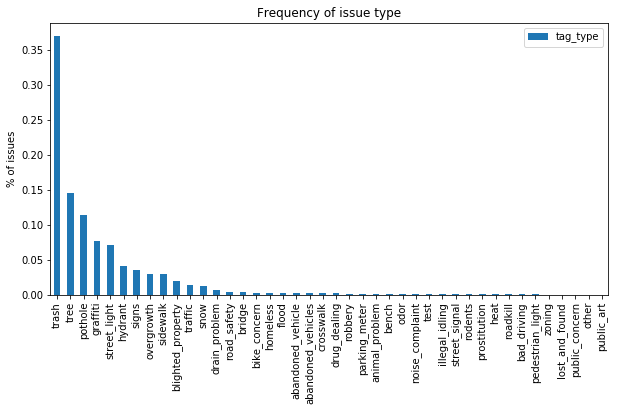
\includegraphics[scale=0.4]{frequency_issue_type}
\par\end{centering}
\caption{Frequency of issue category.}

\end{figure}
One could argue that this order of relevance among issues type would
be enough as prioritization tool, but typically this is hardly the
case. Imagine two situations of fallen trees, one on the sidewalk
and other on the street, blocking the passage. It is easy to estimate
the high urgency of the second case. Even having more and more detailed
categories, it is always possible that exceptions can occur. Thus,
ideally, what we would like to evaluate is if a statistical model
would be able of showing a fine grained distinction between levels
of urgency, based on the features available in the present setting
(of course a platform could allow people to check weather a problem
is urgent or not, but this not the case here). 

\begin{figure}
\begin{centering}
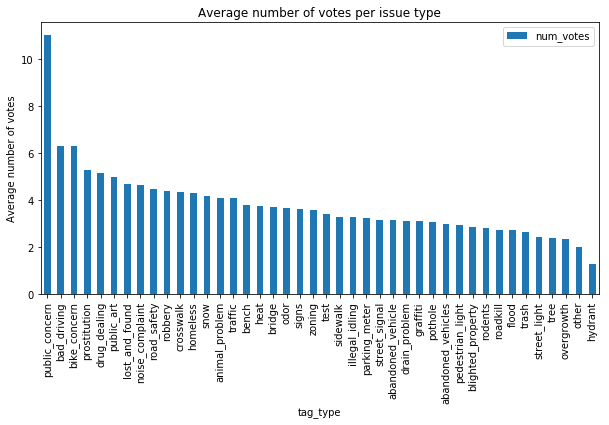
\includegraphics[scale=0.4]{ratio_votes_issue_category}
\par\end{centering}
\caption{Average number of votes per issue type.}
\end{figure}
Finally, Figure 3 shows that more than 70\% of the reported issues
have only one vote. For a crowdsourcing platform, this is not very
encouraging, and we may expect that the data may not be very meaningful
since there is that little variability in \emph{num\_votes}. This
fact may jeopardize our aim of fine grained evaluation since there
are not examples to learn from. 

\begin{figure}
\begin{centering}
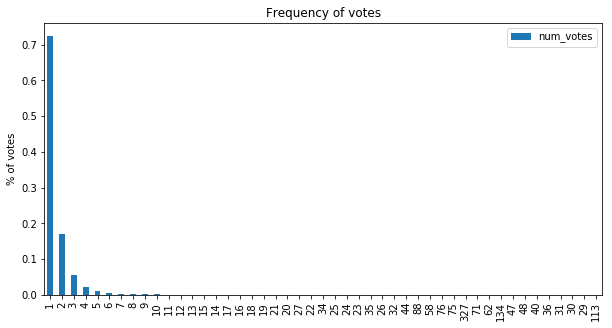
\includegraphics[scale=0.4]{frequency_num_votes}
\par\end{centering}
\caption{Frequency of votes.}

\end{figure}
Another important statistic is the length of the summary and description
fields. This has influence in how to set the parameters of our models
and are depicted in Table 2. The average number of words for summary
are 6.4 words, and for description are 13 words. 

\begin{table}
\begin{centering}
\begin{tabular}{|c|c|c|c|}
\hline 
\textbf{Feature} & \textbf{Max} & \textbf{Min} & \textbf{Avg}\tabularnewline
\hline 
\hline 
Summary & 49 & 1 & 3.04\tabularnewline
\hline 
Description & 924 & 1 & 6.17\tabularnewline
\hline 
\end{tabular}
\par\end{centering}
\caption{Statistics of the summary and description fields}
\end{table}
As we mentioned before, our main goal is to help in estimating the
urgency of a reported issue by predicting \emph{num\_votes}. As evaluation
metric we use the Mean Squared Error (MSE), which evaluates how close
are \emph{p} and \emph{a}, the predicted and the true value. The MSE
formula is given by:

\[
MSE=\frac{1}{n}\sum(p_{i}-a_{i})^{2}
\]

In the next section we discuss in more detail our experiments. We
make a brief description of the algorithms and features we use, and
also show the MSE issued by each of them. 

\section{Experiment and results}

In order to evaluate the feasibility of our proposal, we test our
hypothesis using four different supervised machine learning algorithms
designed to solve regression problems. The overall methodology for
the experiment can be summarized by the following points:
\begin{APAenumerate}
\item Extract suitable features: the features we use to train our models
are description, summary, date and location (latitude and longitude).
We divide the experiment in two parts: 
\begin{APAenumerate}
\item Part A: using only the textual features: summary and description. 
\item Part B: using all four features: summary, description, source and
location.
\item We do that because we want to evaluate how well the models will perform
using only these two attributes. We make the assumption that textual
description features will always be present. Having both results separately
helps to find which model is better in a more general scenario. 
\end{APAenumerate}
\item Configure the parameters and train the models using a training set.
\item The estimated MSE is the mean of a 5-fold cross-validation. 
\end{APAenumerate}
This section is organized as follows: first we describe in more details
how we use the selected features, then we make a brief description
of each algorithm used, and finally we present the results obtained
for Part A and B. 

\subsection{Feature Extraction}

One important matter in using supervised learning algorithms is to
have data in a suitable form to feed them. The task of transform the
raw data in features is called feature extraction and some of the
representation techniques we use are:
\begin{APAitemize}
\item Bag-of-words (BOW): This is the most common approach to extract features
from text. The idea is to represent each document as a (sparse) vector
where each cell counts the number of times a particular word has occurred
in the text. BOW does not consider the order of words and it is often
used with n-gram models. 
\item Word Semantic Vectors: word vectors, Word2Vec, word embedding are
all designations of how has been known the recent supervised learning
technique to learn distributed representation of words \citet{Mikolov:2013:DRW:2999792.2999959}.
The main idea of the skip-gram with negative sampling algorithm is
to train a two layer neural network to predict the probability of
all other words in the vocabulary be in the vicinity of this word.
At the end of the training, the hidden layer will be the word vector
because one way for the network to output similar context predictions
is if the word vectors are similar. So, if two words have similar
contexts, then the network is motivated to learn similar word vectors
for these two words.
\end{APAitemize}
The transformations we apply on the features are:
\begin{APAitemize}
\item prediction and summary: to use with Ridge and SVM, transform to a
BOW representation with 5000 words vocabulary size and pruning words
that occur in more than 50\% of the documents. To use with LSTM we
convert each word in a 200 dimensional word embedding. Fill with a
blank character whenever it is null.
\item date: split in hour, day of week, year, and transform in its one-hot
encoding representation.
\item location: as they are latitude and longitude values represented as
decimal degrees, round to three decimal places which corresponds to
neighborhood precision. Apply one-hot encoding conversion. 
\item log transform \emph{num\_votes} for the linear models.
\end{APAitemize}

\subsection{Algorithms}

Follow a brief description of the algorithms we use: 
\begin{APAitemize}
\item Ridge regression: is a variant of the Ordinary Least Square that applies
a penalty to the loss function in order to prevent from overfitting.
This is achieved by adding an extra term to the loss that is a squared
sum of the weights. This stimulates the optimization procedure to
shrink the weights parameters (but not zeroing them). It is also known
as L2 regularization. 
\item Support Vector Machines (SVM): is a flexible and powerful algorithm
based on the idea of ``large margin''. It builds hyperplanes which
can be used for classification or regression. These hyperplanes are
built in such a way to preserve the larger distance possible between
the samples contained in the two sides being separated. This in turn
implies in lower generalization error. SVM is essentially a linear
model. However, it can be extended to non-linear boundaries by using
different kernels which implicitly transform the original features
using non linear functions. 
\item Long Short Term Memory: is a class of neural models designed to tackle
sequence like problems, i.e., problems where past information is relevant
to compute actual outcomes. Among common problems defined as sequential
are speech recognition, time series analysis, and neural language
models. LSTM is an improved version of a simpler neural model called
Recurrent Neural Network (RNN), Figure 4 left of \citet{Jurafsky:2000:SLP:555733}.
They share the idea of having a time component, a memory, to enable
them to take into account history of information. LSTM is more robust
and complex and is the \emph{de facto} solution as it allows to process
and learn from longer sequences by solving many RNN limitations. The
main drawback of simple RNN is that it uses a single matrix of weights
(the memory component) to compute actual predictions and also to accumulate
past information. Another problem related to neural models in general
is the vanishing or exploding gradients, an intrinsic effect associated
with the way these models learn and that is leveraged in sequence-like
problems as the sequences trend to be lengthy. LSTM tackle these issues
using an intricate mechanism of gates to control the extent to which
a new value flows into a LSTM unit (input gate), the extent to which
a value remains in the unit (forget gate), and the extent to which
a value in the unit is used to compute its output (output gate).
\end{APAitemize}
\begin{figure}
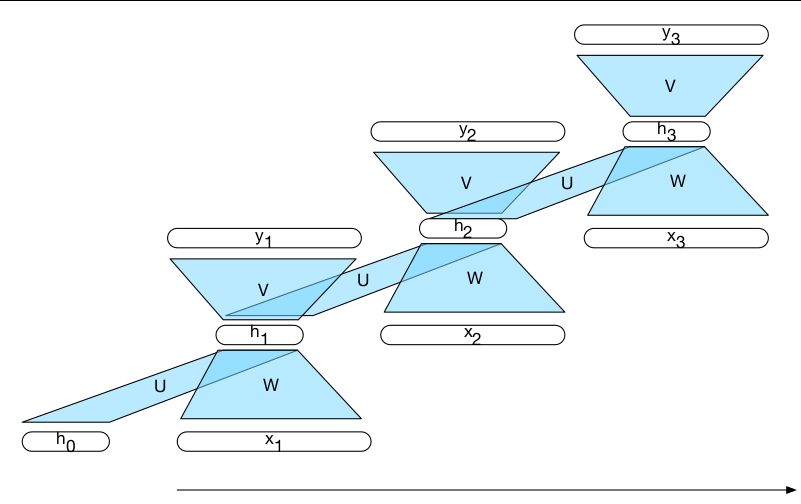
\includegraphics[scale=0.3]{Unroled_RNN}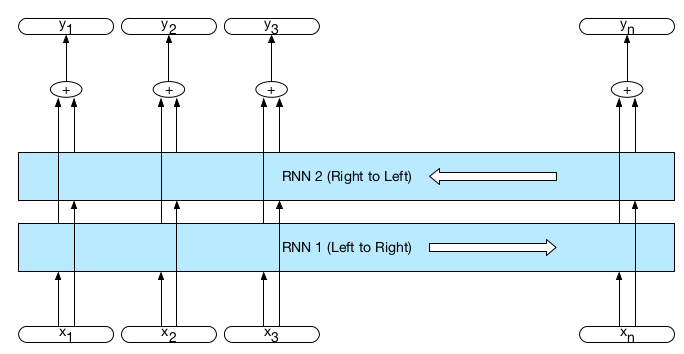
\includegraphics[scale=0.3]{bidirectional_RNN}

\caption{Left: An schematic view of a simple recurrent neural network shown
unrolled in time. Right: A bidirectional RNN. }
\end{figure}
\begin{APAitemize}
\item Bidirectional LSTM: Figure 4 right shows a scheme of a bidirectional
RNN. In a regular RNN (or LSTM) at each step in time the network learned
everything about the sequence up to that point. We say that the model
is taking into account the context in its left. For many problems,
however, we have access to the entire sequence beforehand. It turns
out that it is also valuable and possible to keep track of the context
in the right as well. Then, the network can combine both contexts
and, as a result, modeling a better representation of the data. This
is accomplished by a bidirectional RNN which process the input sequence
from the start to the end, and also in reverse, terribly capturing
left and right contexts into a single representation. There are different
architectures in which we can use Recurrent Neural Networks. For our
proposal, we are using a Many to One design, which means we have as
input a sequence and as output a single value. This scheme is depicted
in Figure 5 (\citet{Jurafsky:2000:SLP:555733}). 
\end{APAitemize}
\begin{figure}
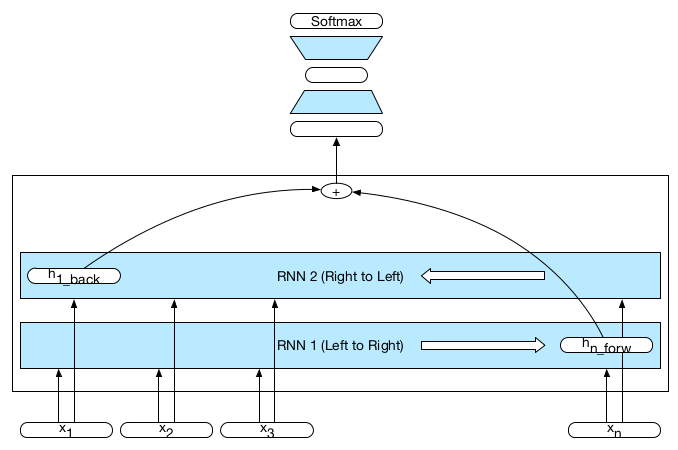
\includegraphics[scale=0.5]{Bi-RNN}

\caption{A bidirectional RNN for sequence classification.}

\end{figure}

\subsection{Experiments and results}

In this section we describe the experiment and the result for each
one of the algorithms experimented. The experiment is divided in two
parts as we want to assess the feasibility of this approach in a more
general setting. Therefore, Part A addresses only textual features
describing the problem. We are assuming that a textual description
of the issue is common among different crowndsourcing platforms. In
Part B we also use location and date as features, as they are available
in SeeClickFix.com data.

However, before we start, as we intend to use linear models to fit
the data, we first test whether the data has a linear relationship.
The graphs in Figure 6 show scatter plots of the residuals and the
predicted values. Such graph can be used to detect if the assumption
of linearity holds. On the left hand side we see the plot over the
original data which has a R-squared of 0.52. The red line is not perfectly
aligned what might mean a non-linear relation. To correct this, we
then apply a log transformation on the target variable. The new plot
on the right has a better fit and a R-squared of 0.673. 

\begin{figure}
\begin{centering}
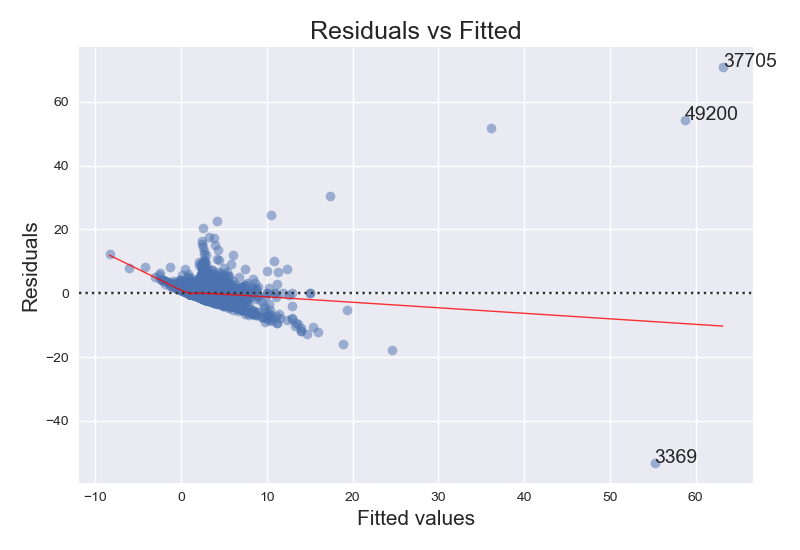
\includegraphics[scale=0.5]{residualxpredicted}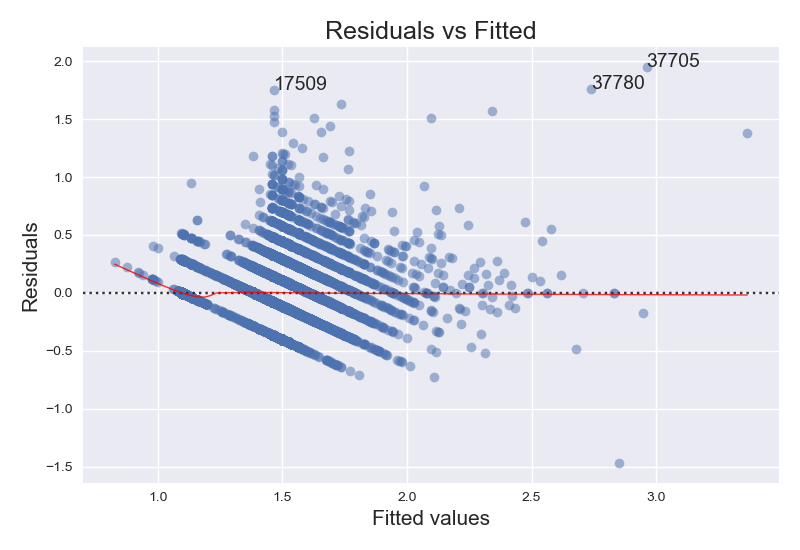
\includegraphics[scale=0.5]{residualxpredicted_}
\par\end{centering}
\caption{Diagnostic Plots}
\end{figure}
These results suggest that a non-linear transformation of the target
variable leads to a better linear model, therefore our experiments
are conducted applying a log-transformation on \emph{num\_votes}. 

\paragraph{Now we present the results for different scenarios. }

Our first set of results, presented in Table 3, encompass the whole
dataset. The table presents, besides the error term, also the R-squared
associated with the linear models. The R-squared, also known as coefficient
of determination, is a metric applied to linear models that captures
the amount of variance of the target variable explained by the predictors.
Thus, for instance, a R-squared of 0.6, means that 60\% of the variability
of Y is explained by X. The results seem to be good, with the LSTM
model being the winner. The MSEs are low and the R-squared are high.
But recall that the variability of the dataset is tiny. Around 72\%
of the examples have only one vote. Thus, if the model only predicts
one, it will be right 72\% of the time. The variance of \emph{num\_votes}
is 1.52. The baseline model here, which predicts the average per neighborhood,
has \textbf{MSE of 0.62}.

\begin{table}
\begin{centering}
\begin{tabular}{|c|c|c|c|c|}
\hline 
\textbf{Algorithm} & \multicolumn{2}{c|}{\textbf{Part A}} & \multicolumn{2}{c|}{\textbf{Part B}}\tabularnewline
\hline 
\hline 
 & \textbf{MSE} & \textbf{R2} & ~\textbf{MSE} & \textbf{R2}\tabularnewline
\hline 
Ridge & 0.86 & 0.59 & 0.82 & 0.60\tabularnewline
\hline 
SVM & 0.87 & 0.40 & 0.85 & 0.40\tabularnewline
\hline 
LSTM & 0.82 & x & 0.65 & x\tabularnewline
\hline 
\end{tabular}
\par\end{centering}
\caption{Results for the complete dataset.}
\end{table}
For the second scenario, we compute the baseline model by predicting
the average of votes grouped by issue type and location. Hence, for
each example, the prediction is the mean computed for that specific
neighborhood and problem category. This model encompasses only the
records whose have \emph{tag\_type} populated (24\% of the data) and
has a \textbf{MSE of 0.83}. Table 4 brings the result for the algorithms
applied to this restricted dataset. Here, the variance of \emph{num\_votes}
is higher (3.41), and the results are much worse. Without using \emph{tag\_type}
as predictor, the latent information present is not enough to the
evaluated models to extract meaningful patterns in order to make an
accurate prediction. Again, the winner was LSTM but still could not
surpass the baseline model. 

\begin{table}
\begin{centering}
\begin{tabular}{|c|c|c|c|c|}
\hline 
\textbf{Algorithm} & \multicolumn{2}{c|}{\textbf{Part A}} & \multicolumn{2}{c|}{\textbf{Part B}}\tabularnewline
\hline 
\hline 
 & \textbf{MSE} & \textbf{R2} & ~\textbf{MSE} & \textbf{R2}\tabularnewline
\hline 
Ridge & 2.87 & 0.13 & 2.70 & 0.18\tabularnewline
\hline 
SVM & 3.01 & 0.1 & 2.81 & 0.16\tabularnewline
\hline 
LSTM & 2.60 & x & 2.33 & x\tabularnewline
\hline 
\end{tabular}
\par\end{centering}
\caption{Results for the baseline dataset.}
\end{table}

\section{Conclusion}

In this work we use machine learning to leverage city maintenance
capabilities. Our hypothesis is that would be possible, with certain
degree of accuracy, to estimate the number of votes an issue would
receive based on their attributes. The number of votes can be used
to estimate urgency and therefore is a useful metric to help in planning
and prioritization. 

To evaluate our hypothesis we employ different machine learning algorithms
with different properties in an attempt to finding the one that suites
better to the data and leads to the most accurate prediction. This
is a common methodology in data analysis since the ground truth function
which generates the data is missing and our goal is to meet an approximation
to it. We explore four regularized linear models - Ridge and SVM -
and a neural model designed to handle sequence learning problems,
LSTM. Linear models are the building blocks of data driven statistical
learning due their maturity, interpretability and predictive power.
The model that issued the smallest error was the neural one. Neural
models are highly flexible and, in this problem, where the main feature
are sentences in the English language, our choice of LSTM performed
pretty well. 

Our findings show that the models could not overcome the baseline
models in both scenarios. In the first one, although the error was
close to the baseline error, there is the issue of the dataset being
biased and have only one vote for around seventy percent of the records.
For the second scenario the baseline, besides the neighborhood, also
uses the category of each problem to compute the predictions. The
size of the dataset decreases and so the accuracy of the models. To
mimic the baseline, the models should have to be inferred the category
from the textual features, which is hard. In both cases the models
were highly dependent on the availability and quality of the textual
information and it seems that regression problems relying on text
is hard. Our findings are inconclusive whether or not machine learning
can be better than simple aggregation and summarization of the data
in this setting. Maybe a better approach would be to use synthetic
data in order to evaluate the real feasibility. 

\bibliographystyle{apacite}
\bibliography{bibliography,sample}

\end{document}
